\ifx\wholebook\relax\else
\input{../Common.tex}
\input{../macroes.tex}
\begin{document}
\fi


\chapter{A Digital Animal: A gluttonous Tomagoshi}\label{cha:toma}

%\begin{chapterfigure}
%\includegraphics[width=\linewidth]{ballInField}
%\end{chapterfigure}

In this chapter we propose you to develop a small digital animal that has its own life require care for you. 
People were really found of digital animals called tomagoshi. Therefore  we will build one step by step. 
This project is a pretext for revisiting the basic actions to define a class, instance variables and methods. 

\section{A gluttonous Tomagoshi }
%%%%%%%%%%%%%%%%%%%%%%%%%%%%%%%%%%%%%%%%%%%%%%
%%%%%%%%%%%%%%%%%%%%%%%%%%%%%%%%%%%%%%%%%%%%%%

We have to decide the behavior that our digital beats should have. 
Here is the list of the behavior we propose you to implement for our  tomagoshi. The Figure~\ref{fig:tomastate} represents how the tomagoshi changes its state. 
\begin{itemize}
\item It can eat and digest food. It can be hungry when its tummy is empty and satisfied when it eats enough food.
\item It has its own life cycle with its own isNights and days. It goes to sleep at isNight and wake up the morning. 
\item It is gluttonous and selfish so falls asleep as soon as it eats enough. 
\item Its change color depending on its mood.  
We choose to have blue when it is  satisfied possibly sleeping, black when sleeping but hungry, green when waking up, and red when it is hungry. 
\end{itemize}

\begin{figure}
\begin{center}
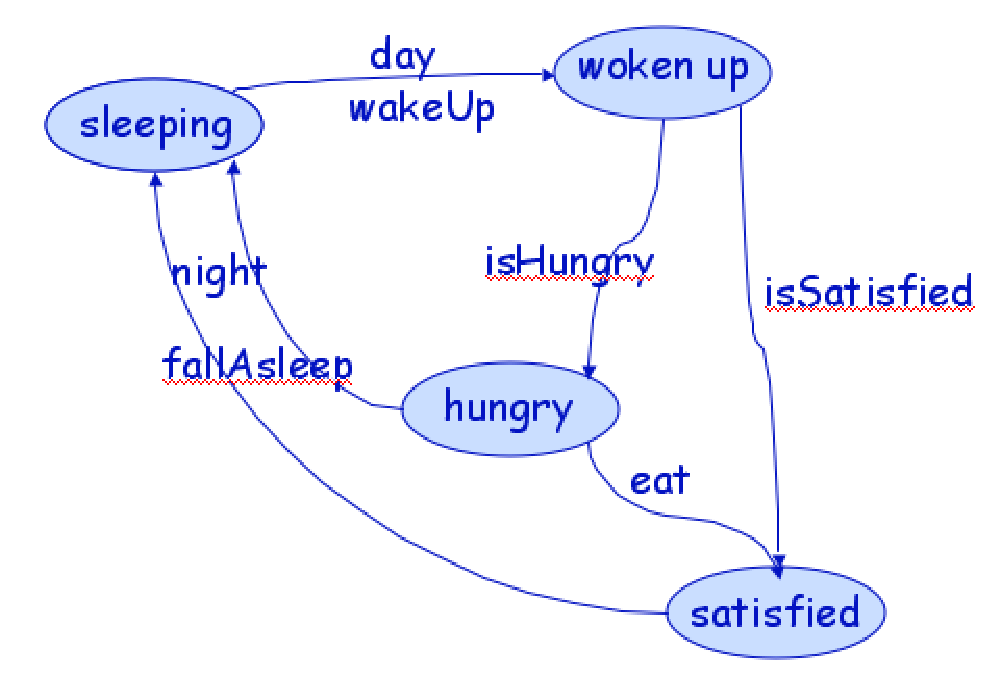
\includegraphics[width=8cm]{tomastate}
\caption{\label{fig:tomastate}}
\end{center}
\end{figure}

\section{Representing Day and isNight Passing}
The first thing we want to represent is the time passing and the alternation of isNights and days.
To represent the time passing, the length of isNights and days and the change between days and isNights we propose you to use two instance variables: \ct{dayCount} and \ct{isNight} defined in the class \ct{Tomagoshi}. 

To model isNight and day passing we have the idea that \ct{dayCount} will hold a number represents the number of hours (or tick) left in the isNight or day. This number will decrease regurlarly and when arriving at zero the isNight or day will end and a new will start. We will use \ct{isNight} as a boolean  representing the fact that this is the isNight.

Define a new class category named for example 'TOMA' and define the class \ct{Tomagoshi}. As we would like to be able to interact with it and have a graphical representation, we define  the class  \ct{Tomagoshi} as a subclass of the class \ct{Morph}. 

\begin{classdef}\label{cls:tomaOne}
Morph subclass: #Tomagoshi
   instanceVariableNames: ' dayCount isNight'
   classVariableNames: ''
   poolDictionaries: ''
   category: 'TOMA'
\end{classdef}

We edit the class comment by pressing the ? button and write something in the vein of:
\begin{alltt}
I represent a tomagoshi. A small virtual animal that have its own life.

dayCount <Number> represents the number of hour (or tick) in my day and night.
isNight <Boolean> represents the fact that this is the night.
\end{alltt}


As done previously in chapter @@, we define the method \ct{initializeToStandAlone} to invoke the ones of the superclasses, this way we will be able to create a graphical object. We also initialize the instance variables \ct{dayCount} and \ct{isNight} by calling a newly created method called \ct{dayStart}. We choose the number 10 as the length of a day or isNight. 


\begin{method}\label{mth:initOne}\cat{initialize}
\textbf{Tomagoshi>>initializeToStandAlone}
   "Initialize the internal state of a newly created tomagoshi"

   super initializeToStandAlone.
   self dayStart.
\end{method}

\begin{method}\label{mth:initOne}\cat{initialize}
\textbf{Tomagoshi>>dayStart}

   isNight := false.
   dayCount := 10
\end{method}

Now we need a way to regularly makes the time passing by decreasing the \ct{dayCount} instance variables. 
The method \ct{step} that is offered by the class \ct{Morph}, is called by the system at regular time interval 
(specified in milliseconds by the method \ct{steppingTime}). Therefore we specialize this method (see 'mthref{tomastepone})
 so that it invokes a newly created method called \ct{timePass} (see \mthref{mth:timePassOne}).

\begin{method}\label{mth:tomastepone}\cat{stepping}
\textbf{Tomagoshi>>step}

   self timePass
\end{method}

\begin{method}\label{mth:}\cat{stepping}
\textbf{Tomagoshi>>steppingTime}

   ^ 500
\end{method}

The method \ct{timePass} makes a beep, then decrease the value of the instance variable \ct{dayCount}, check whether the 
time period is over, if this is the case it reinitialize it and update the instance variable \ct{isNight} to represent  the new period. This last action is done by the method \ct{isNightOrDayEnd} (see \mthref{mth:isNightOrDayEnd}). 

\begin{method}\label{mth:timePassOne}\cat{day and isNight}
\textbf{Tomagoshi>>timePass}
   "Manage the isNight and day alternance"

   Smalltalk beep. 
   dayCount := dayCount -1.
   dayCount isZero
      ifTrue:
          [ self isNightOrDayEnd. 
          dayCount := 10]
\end{method}

\begin{method}\label{mth:isNightOrDayEnd}\cat{day and isNight}
\textbf{Tomagoshi>>isNightOrDayEnd}
  "alternate isNight and day"

   isNight := isNight not
\end{method}


\section{Adding Behavior}
Now we should represent the state of our animal, if it is sleeping, hungry, and how it will changes its emotions. 
Our digital animal is mainly occupied to satisfied its hunger.  We add two instance variables to represent the appetite of our small beast. The instance variable \ct{tummy} represents the amount of food that the tomagoshi ate. The instance variable \ct{hunger} represents its appetite. It will only be satisfied when it tummy is higher than its hunger. 


\begin{classdef}\label{cls:tomaTwo}
Morph subclass: #Tomagoshi
   instanceVariableNames: ' dayCount isNight tummy hunger'
   classVariableNames: ''
   poolDictionaries: ''
   category: 'TOMA'
\end{classdef}



We update the class comments with the following information.
\begin{alltt}
tummy <Number> represents the number of times you feed me by clicking on me.
hunger <Number> represents my appetite power. 
I will be hungry if you do not feed me enough, but I'm selfish so as soon as I' satisfied I fall asleep because I do not have a lot to say. 
\end{alltt}

We change the \ct{initializeToStandAlone} method to initialize the tummy to zero to state that it did not ate, and we choose to set its hunger randomly between 1 and 3. (the method \ct{Integer>>atRandom} returns a random number between the 1 and the receiver). 

\begin{method}\label{mth:InitializeTwo}\cat{initialize}
\textbf{Tomagoshi>>initializeToStandAlone}
    "Initialize the internal state of a newly created tomagoshi"

   super initializeToStandAlone.
   \textbf{tummy := 0.
   hunger := 3 atRandom.}
   self dayStart.
\end{method}



Then we define the method \ct{eat} as simply incrementing the number of item eaten. The method \ct{digest} as decrementing this number by one. However, we consider digesting a slower process than eating so we one decrement the contents of the \ct{tummy} instance variable when the clock represented by \ct{dayCount} value is even (here we use \ct{isDivisibleBy: 2} because this way you can model different animal easily, the method \ct{even} would have worked) (see \mthref{mth:digest}). 


\begin{method}\label{mth:eat}\cat{behavior}
\textbf{Tomagoshi>>eat}
   tummy := tummy + 1
\end{method}

\begin{method}\label{mth:digest}\cat{behavior}
\textbf{Tomagoshi>>digest}
   "Digest slowly: every two cycles, remove one from the tummy"

   (dayCount isDivisibleBy: 2)   
      ifTrue: [ tummy := tummy -1]
\end{method}

As the digestion is a process that is linked with time, we call the method \ct{digest} from the method \ct{timePass} as shown in \mthref{mth:timePassThree}.

\begin{method}\label{mth:timePassThree}\cat{day and isNight}
\textbf{Tomagoshi>>timePass}
   "Manage the isNight and day alternance"

   Smalltalk beep. 
   dayCount := dayCount -1.
   dayCount isZero
      ifTrue:
         [self isNightOrDayEnd. 
         dayCount := 10].
   \textbf{self digest}
\end{method}


\begin{figure}
\begin{center}
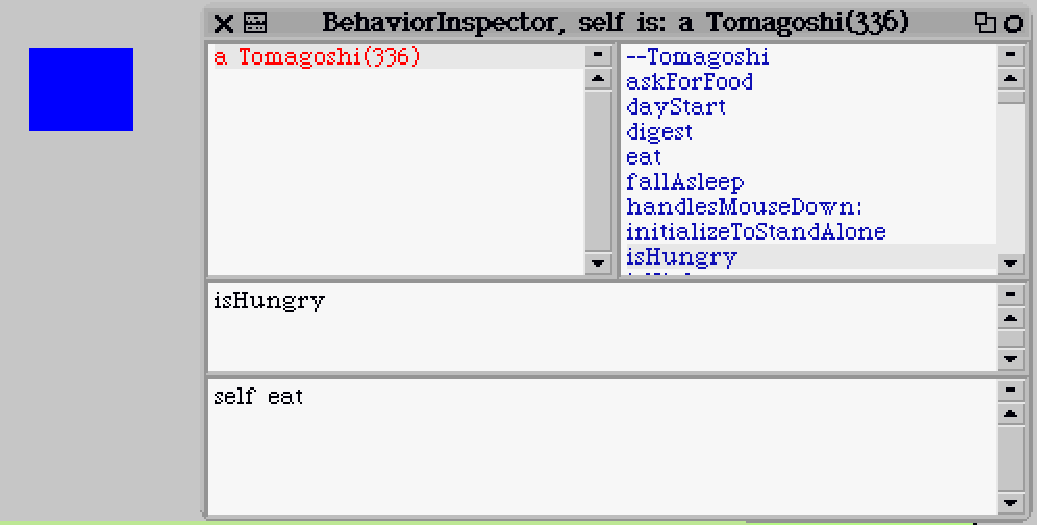
\includegraphics[width=10cm]{toma}
\caption{The tomagoshi inspected using the behavioral inspector. The right pane shows all the methods the object selected in the right pan understand. The bottom pane allows one to define methods or execute expression. The middle pane show the message definition and its comment. \label{fig:toma}}
\end{center}
\end{figure}

Now we define two methods \ct{isHungry} and \ct{isSatisfied} that returns whether the tomagoshi is hungry or not. 

\begin{method}\label{mth:isHungry}\cat{behavior}
\textbf{Tomagoshi>>isHungry}
   ^ hunger > tummy 
\end{method}

\begin{method}\label{mth:isSatisfied}\cat{behavior}
\textbf{Tomagoshi>>isSatisfied}
   ^self isHungry not
\end{method}

Now we need to be able to wake up our tomagoshi, so we define the method \ct{wakeUp} (see~\mthref{mth:wakeUp}). This method changes its color and its state. For the state representation, as we do not wanted to duplicate the way the state is represented we define two methods \ct{wakeUpState} (see \mthref{mth:wakeUpState}) which returns the internal representation associated to the state waking up. The method~\mthref{mth:isSleeping} returns whether the tomagaoshi is sleeping and again we do not code directly the fact that waking up state is code as the symbol \ct{\#sleep} but use the method \ct{wakeUpState} that defines this representation. Hence we will be able to change the representation by just changing one method and not three. 

\begin{method}\label{mth:wakeUp}\cat{behavior}
\textbf{Tomagoshi>>wakeUp}
   self color: Color green.
   state := self wakeUpState
\end{method}

\begin{method}\label{mth:wakeUpState}\cat{behavior}
\textbf{Tomagoshi>>wakeUpState}
  "Return how we codify the fact that I sleep"
   ^ #sleep
\end{method}

\begin{method}\label{mth:isSleeping}\cat{behavior}
\textbf{Tomagoshi>>isSleeping}
   ^ state = self wakeUpState
\end{method}

Now we have nearly all the behavior defined, so we are ready to complete the method \ct{step} as presented in \mthref{mth:stepTwo}.

\begin{method}\label{mth:stepTwo}\cat{stepping}
\textbf{Tomagoshi>>step}
  "This method is called by the system at regurlar time interval.
   It defines the tomagoshi behavior."

   self timePass.
   \textbf{self isHungry
      ifTrue: [self color: Color red].
   self isSatisfied
      ifTrue: 
         [self color: Color blue.
         self fallAsleep].
   self isNight 
      ifTrue: 
         [self color: Color black. 
         self fallAsleep]}
\end{method}

To work we still have to define the method \ct{isNight} as shown in \mthref{mth:isNight}.Note that we could have use the instance variable
\ct{isNight} directly but this would have been breaking the rythm or abstraction level of the  method body as we do not use direct access to instance variable at all in this method. 

\begin{method}\label{mth:isNight}\cat{day and isNight}
\textbf{Tomagoshi>>isNight}
   ^ isNight
\end{method}

Finally we just have to adapt slightly the \ct{initializeToStandAlone} method so that a newly created tomagoshi is woken up. 

\begin{method}\label{mth:InitializeThree}\cat{initialize}
\textbf{Tomagoshi>>initializeToStandAlone}
    "Initialize the internal state of a newly created tomagoshi"

   super initializeToStandAlone.
   tummy := 0.
   hunger := 2 atRandom + 1.
   self dayStart.
   \textbf{self wakeUp}
\end{method}

\begin{figure}
\begin{center}
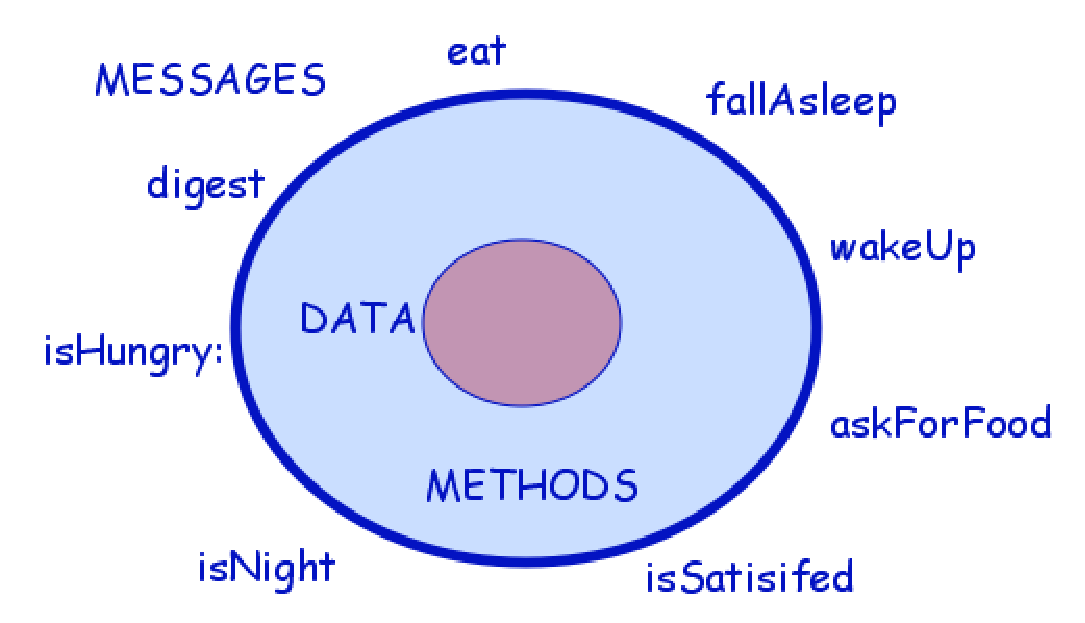
\includegraphics[width=10cm]{messageOnly}
\caption{A tomagoshi. It proposes to the rest of the world a list of messages representing its 
behavior, \textit{i.e.,} what he can do. From outside the tomagoshi its internal representation is not visible\label{fig:messageOnly}}
\end{center}
\end{figure}


Now we would like to be able to feed the tomagoshi just by clicking on it so we just define the two following methods (see \mthref{mth:tomahandlesMouseDown} and \mthref{mth:tomamouseDown}. These methods are fully explained in the chapter @@. 

\begin{method}\label{mth:tomahandlesMouseDown}\cat{stepping}
\textbf{Tomagoshi>>handlesMouseDown: evt}
   "true means that the morph can react when the mouse down over it"
   ^ true
\end{method}

\begin{method}\label{mth:tomamouseDown}\cat{stepping}
\textbf{Tomagoshi>>mouseDown: evt}
    self eat
\end{method}


\section{Further Experiments}
Now we propose you different modifications to change the behavior of your tomagoshi. 

\begin{itemize}
\item Make that we can only feed the tomagoshi the day. 
\item Make it die when it is starving from too long time (hints you can use the method 
\ct{delete} or \ct{stopStepping}).
\item Make it happy after lunch and not only falling asleep. You could make it sings.
\item Change its graphical representation.  
\item Using the method \ct{PopUpMenu inform: aString} that pop up a menu, make
 the tomagoshi ask for food. 
\item Define the method \ct{printOn: aStream} so that we see the state of the
 tomagoshi in inspector or when sending a \ct{printString} message to a tomagoshi. The
 new displayed string could be \ct{'a Tomagoshi (98987) with state: asleep'} instead of
 what we have now:  \ct{'a Tomagoshi (98987)'}
\end{itemize}

\paragraph{Improving the code.} \ct{dayCount := 10} is duplicated in several places. If we want to
 change the length of the day we will have to change this constant in lot of places. Change this
 situation so that we only have this logic in one place. 

\begin{figure}
\begin{center}
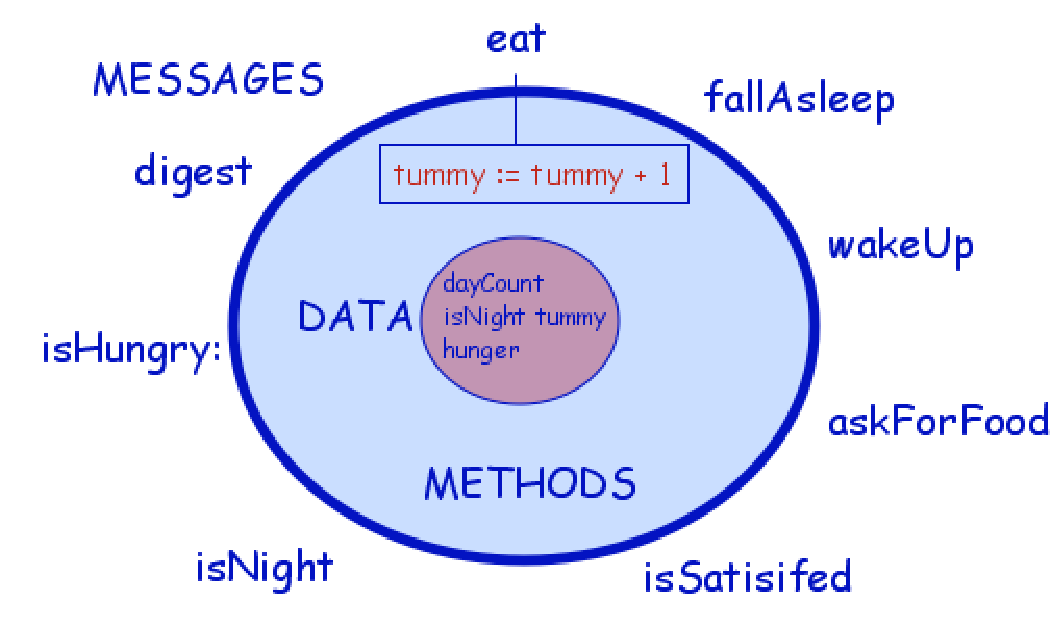
\includegraphics[width=10cm]{full}
\caption{An object presents an interface composed by a set of messages defining \textit{what} the object can do. This behavior is realized by methods that specify \textit{how} the behavior is implemented. To realize the behavior, data is most of the time required. The data is only accessed by the methods. \label{fig:full}}
\end{center}
\end{figure}


\section{What the Example Shows}
We hope that implementing a tomagoshi was certainly a fun experiment. However this is more than that. Now we will look at all the lessons
we can learn from it. 


\paragraph{Messages vs. Methods: What vs. How.} The tomagoshi implementation illustrates the difference between messages\index{messages} and \index{methods} methods. A message represents \textit{what} an object is capable to do. It is composed by a list of actions. 
In the figure\ref{fig:messageOnly}, the messages are all the behavior of the tomagoshi such as \ct{eat}, \ct{digest}, \ct{wakeUp}... Methods define \textit{how} the behavior described by the message is actually specified. The Figure~\ref{fig:full} shows that the message \ct{eat} is realized by the method \ct{eat}. As we decided to represent the tummy 
of a tomagoshi using just one number representing the number of items the tomagoshi ate, the \textit{method} \ct{eat}
increments the \ct{tummy} instance variables. 




\paragraph{\index{Encapsulation}Encapsulation.} The example illustrates that the data hold in instance variable is private to the object. Only its methods can access them. In fact as someone interacting with the tomagoshi we do not have to know how it is internally defined. We are only interested by the messages that we can send to it. We say that the data is encapsulated. What encapsulation provides is that we can continue to interact with the
tomagoshi using the same messages even if its internal representation changes. We can rely on its messages.
For example, we used two instance variables one for the tummy and one for the hunger of the tomagoshi. Other implementation strategies can still provides the same interface (set of messages) while changing the number and roles of instance variables. 


\paragraph{Factoring Logic.}
At the code level the example shows how the internal representation of certain state can be factored and only expressed in one place. Hence the method \ct{wakeUpState} which returns a symbol (see~\mthref{mth:wakeUpState}) is the only one that defines how the state is represented. This means that we can change it freely. In our case this is not important but we could. This avoid to duplicate this knowledge all over the places. This follow the rule "Say once and only once". 












\ifx\wholebook\relax\else
\end{document}\fi
